\begin{apendicesenv}

\chapter{Descrição do Processo de ETL no Kettle}
\label{sec:implementação-etl}

Neste apêndice, será apresentado a implementação do ETL no Kettle, onde se utilizou dos arquivos CSV resultantes da análise de métricas de código-fonte do Analizo. Embora, o Kettle tivesse componentes de interpretação dos elementos de CSV, no presente trabalho, decidiu-se por converter CSV obtido do Analizo em arquivos JSON, visto que componente de CSV do Kettle, converte-o para XML, sendo que este é mais lento e menos versátil quando comparado ao JSON, tal como se mostra no trabalho de \citeonline{fonseca2007alternativas}. Visando realizar a conversão, foi escrito um pequeno \textit{parser} na linguagem \textit{Ruby}, tal como se vê no Código-Fonte \ref{Ruby}.

\begin{center}
\begin{minipage}{0.5\textwidth}
\lstinputlisting[caption=\textit{Parser} de CSV para JSON, language=Ruby, label=Ruby]{codigos/parser.rb}
\end{minipage}
\end{center}

\section{Implementações das \textit{Transformations}}


Como explicado anteriormente, o Kettle utiliza o componente de \textit{Transformation} para realizar cálculos, consultas em tabelas, inserções em tabelas, leitura de dados e entre outros. Alguns desses componentes são mostrados na Figura \ref{fig:components-etl}.


\begin{figure}[H]
\centering
\includegraphics[keepaspectratio=false,scale=0.60]{figuras/components-transformation.eps}
\caption{Componentes do Kettle que foram utilizadas nas Transformações}
\label{fig:components-etl}
\end{figure}
\FloatBarrier

O componente \textit{JSON Input} serve para ler os dados provenientes de um arquivo JSON, em que o conteúdo de cada variável pode ser lido como: \$..@nome\_da\_variavel. O componente \textit{Univariate Statistics} é utilizado para se calcular estatísticas como média, mediana, número de amostras e percentis, que foram utilizados no cálculo dos intervalos percentis das métricas de código-fonte; O componente \textit{Execute SQL Script} foi utilizado para recuperação de dados no Metadados e Dimensões e também para inserção de nas Tabelas Fatos; O componente \textit{Combination Lookup} foi utilizado para se verificar se um determinado já exisitia em uma Dimensão, caso existisse, apenas se retornava o id da túpula, se não o inseria na Dimensão; Por fim o componente \textit{Select Values} foi utilizado para filtrar os dados provienente de outros componentes em uma \textit{Transformation}.


Na primeira transformação, como se mostra na Figura \ref{fig:first-transformation}, obtém-se os dados provinientes do arquivo JSON com componente \textit{JSON Input}. Em uma primeira etapa, coletava-se sobre dados: nome do projeto, release do arquivo, data de lançamento da release. Após a coleta dos dados do arquivo JSON, se inseria, conforme as verificações do componente \textit{Combination Lookup}, nas dimensões correspondentes.


\begin{figure}[H]
\centering
\includegraphics[keepaspectratio=false,scale=0.65]{figuras/first-transformation.eps}
\caption{Primeira Transformação realizada no Kettle}
\label{fig:first-transformation}
\end{figure}
\FloatBarrier

Na segunda transformação, como se mostra na Figura \ref{fig:second-transformation}, cobre-se o processo de negócio de avaliação dos valores percentis das métricas de código-fonte do projeto em uma determinada \textit{release} do software. Para tal, foi coletado os valores das métricas de código-fonte de cada classe com o componente \textit{JSON Input}. Após a coleta dos valores das métricas, esses eram direcionados ao componente \textit{Univariate Statistics} que realiza cálculos estatísticos. Após a realização dos cálculos, foi realizado um filtro com \textit{Select Values} a fim de se obter apenas os percentis obtidos para cada umas das métricas. 

\begin{figure}[H]
\centering
\includegraphics[keepaspectratio=false,scale=0.65]{figuras/second-transformation.eps}
\caption{Segunda Transformação realizada no Kettle}
\label{fig:second-transformation}
\end{figure}
\FloatBarrier

Por fim, foi realizado a avaliação dos valores percentis, em intervalos qualitativos nos metadados com o componente \textit{Execute SQL Script}. Neste componente, recebeu-se o código-fonte descrito no Código-Fonte \ref{sql-etl-project}, onde cada \? foi substuído por uma variável dentro da \textit{Transformation}.

\lstinputlisting[caption=\textit{Script} SQL de Avaliação dos Valores Percentis das Métricas de Código-Fonte, language=SQL, label=sql-etl-project]{codigos/project-fact.sql}

Na terceira trasnformação, como se mostra na Figura \ref{fig:third-transformation}, foram cobertos os procesos de negócio de avaliar os cenários de limpeza de código-fonte em cada classe do Projeto em uma determinada \textit{release} e o cálculo da Taxa de Aproveitamento de Oportunidades de Melhoria de Código-Fonte. Para tal, foram obtidos os valores cada métrica para cada classe utilizando o componente \textit{JSON Input}. Após a coleta das métricas, foram inseridas, utilizando o componente \textit{Combination Lookup} a fim de evitar duplicações ao longo das \textit{releases}, as classes do projeto.


\begin{figure}[H]
\centering
\includegraphics[keepaspectratio=false,scale=0.65]{figuras/third-transformation.eps}
\caption{Terceira Transformação realizada no Kettle}
\label{fig:third-transformation}
\end{figure}
\FloatBarrier

Por fim, foram identificados os Cenários de Limpeza de Código-Fonte com auxílio dos metadados utilizando o componente \textit{Execute SQL Script}. Aind neste componente, foi calculada a Taxa de Aproveitamento de Oportunidades de Melhoria de Código-Fonte a partir a soma de todos cenários de limpeza identificados em uma determinada release e a soma de todas as classes. O código-fonte, que foi colocado no componente \textit{Execute SQL Script} é descrito no Código-Fonte \ref{sql-etl-class}, onde cada \? foi substuído por uma variável dentro da \textit{Transformation}.

\lstinputlisting[caption=\textit{Script} SQL de Identificação de Cenários de Limpeza de Código-Fonte e Cálculo da Taxa de Aproveitamento de Oportunidades de Melhoria de Código-Fonte, language=SQL, label=sql-etl-class]{codigos/class-fact.sql}


\section{Implementação do \textit{Job}}

Como explicado anteriormente, o Kettle utiliza o  \textit{Job} para executar tarefas, em nível mais alto, de fluxo de controle, tais como, mandar um email em caso de falha, baixar um arquivo, executar transformações  e entre outras atividades. Dessa forma os principais componentes internos do \textit{Job}, que foram utilizados no trabalho, são mostrados na Figura \ref{fig:components-job}. 

\begin{figure}[H]
\centering

\includegraphics[keepaspectratio=false,scale=0.60]{figuras/componentes-job.eps}
\caption{Componentes do Kettle que foram utilizadas nos \textit{Jobs}}
\label{fig:components-job}
\end{figure}
\FloatBarrier

O componente \textit{Start} é utilizado para marcar o início da execução de um determinado \textit{Job}. Nele, é possível programar a execução repetida de um determinado \textit{job}, como por exemplo, a cada hora, dia ou mês; Já o componente \textit{Transformation} serve para executar uma determinada Transformação, que fora especificada anteriormente.

Após se contruir o arquivo \textit{Job} do presente trabalho, obteve-se a Figura \ref{fig:job}. 

\begin{figure}[H]
\centering
\includegraphics[keepaspectratio=false,scale=0.60]{figuras/job.eps}
\caption{\textit{Job} deste Trabalho}
\label{fig:job}
\end{figure}
\FloatBarrier

No \textit{Job}, a transformação~"Dados do Projeto"~corresponde a execução da Figura \ref{fig:first-transformation}. Já a transoformação~"Análise dos Valores Percentis"~corresponde a Figura \ref{fig:second-transformation} e por fim, a transformação~"Análise dos Cenários de Limpeza de Código-Fonte" corresponde a Figura \ref{fig:third-transformation}.

\chapter{Gráficos e Tabelas dos Percentis de Métricas de Código-Fonte}

Neste apêndice, serão apresentados os gráficos e tabelas, obtidos com o plugin Saiku no ambiente de \textit{Data Warehousing}, dos Percentis obtidos para cada uma das métricas de código-fonte no Sistema Integrado de Conhecimento e Gestão (SICG) do Instituto do Patrimônio Arstítico Nacional (IPHAN).

\label{graphs}

\begin{sidewaysfigure}[h]
\centering
\includegraphics[scale=0.70]{figuras/acc-grafico.eps}
\includegraphics[scale=0.70]{figuras/acc-tabela.eps}
\caption{Intepretação dos Valores Percentis da Métrica ACC}
\label{fig:metric-acc}
\FloatBarrier
\end{sidewaysfigure}

\begin{sidewaysfigure}[h]
\centering
\includegraphics[scale=0.70]{figuras/accm-grafico.eps}
\includegraphics[scale=0.70]{figuras/accm-tabela.eps}
\caption{Intepretação dos Valores Percentis da Métrica ACCM}
\label{fig:metric-accm}
\FloatBarrier
\end{sidewaysfigure}

\begin{sidewaysfigure}[h]
\centering
\includegraphics[scale=0.70]{figuras/amloc-grafico.eps}
\includegraphics[scale=0.70]{figuras/amloc-tabela.eps}
\caption{Intepretação dos Valores Percentis da Métrica AMLOC}
\label{fig:metric-amloc}
\FloatBarrier
\end{sidewaysfigure}

\begin{sidewaysfigure}[h]
\centering
\includegraphics[scale=0.75]{figuras/anpm-completo.eps}
\includegraphics[scale=0.70]{figuras/anpm-projeto.eps}
\caption{Intepretação dos Valores Percentis da Métrica ANPM}
\label{fig:metric-anpm}
\FloatBarrier
\end{sidewaysfigure}

\begin{sidewaysfigure}[h]
\centering
\includegraphics[scale=0.70]{figuras/cbo-grafico.eps}
\includegraphics[scale=0.70]{figuras/cbo-tabela.eps}
\caption{Intepretação dos Valores Percentis da Métrica CBO}
\label{fig:metric-cbo}
\FloatBarrier
\end{sidewaysfigure}

\begin{sidewaysfigure}[h]
\centering
\includegraphics[scale=0.70]{figuras/dit-grafico.eps}
\includegraphics[scale=0.70]{figuras/dit-tabela.eps}
\caption{Intepretação dos Valores Percentis da Métrica DIT}
\label{fig:metric-dit}
\FloatBarrier
\end{sidewaysfigure}



\begin{sidewaysfigure}[h]
\centering
\includegraphics[scale=0.45]{figuras/lcom4-projeto.eps}
\includegraphics[scale=0.5]{figuras/lcom4-completo.eps}
\caption{Intepretação dos Valores Percentis da Métrica LCOM4}
\label{fig:metric-LCOM4}
\FloatBarrier
\end{sidewaysfigure}


\begin{sidewaysfigure}[h]
\centering
\includegraphics[scale=0.70]{figuras/loc-grafico.eps}
\includegraphics[scale=0.70]{figuras/loc-tabela.eps}
\caption{Intepretação dos Valores Percentis da Métrica LOC}
\label{fig:metric-loc}
\FloatBarrier
\end{sidewaysfigure}

\begin{sidewaysfigure}[h]
\centering
\includegraphics[scale=0.70]{figuras/noc-grafico.eps}
\includegraphics[scale=0.70]{figuras/noc-tabela.eps}
\caption{Intepretação dos Valores Percentis da Métrica NOC}
\label{fig:metric-noc}
\FloatBarrier
\end{sidewaysfigure}

\begin{sidewaysfigure}[h]
\centering
\includegraphics[scale=0.70]{figuras/nom-grafico.eps}
\includegraphics[scale=0.70]{figuras/nom-tabela.eps}
\caption{Intepretação dos Valores Percentis da Métrica NOM}
\label{fig:metric-nom}
\FloatBarrier
\end{sidewaysfigure}

\begin{sidewaysfigure}[h]
\centering
\includegraphics[scale=0.70]{figuras/npa-grafico.eps}
\includegraphics[scale=0.70]{figuras/npa-tabela.eps}
\caption{Intepretação dos Valores Percentis da Métrica NPA}
\label{fig:metric-npa}
\FloatBarrier
\end{sidewaysfigure}

\begin{sidewaysfigure}[h]
\centering
\includegraphics[scale=0.70]{figuras/rfc-grafico.eps}
\includegraphics[scale=0.70]{figuras/rfc-tabela.eps}
\caption{Intepretação dos Valores Percentis da Métrica RFC}
\label{fig:metric-rfc}
\FloatBarrier
\end{sidewaysfigure}

\chapter{Cenários de Limpeza de Código-Fonte}
\label{scenarios}

Neste apêndice, são detalhadas as classes e os cenários de limpeza de código-fonte que foram identificados para as mesmas ao longo das \textit{releases} do projeto. 

\begin{table}[H]
\centering
\input{tabelas/resultados-cenarios-metodo-grande.ltx}
\caption{Classes com Cenário de Limpeza: Classe com métodos muito grandes e/ou muitos condicionais}
\end{table}

\begin{table}[H]
\centering
\input{tabelas/resultados-cenarios-filhos.ltx}
\caption{Classes com Cenário de Limpeza: Classe com muitos filhos}
\end{table}

\begin{table}[H]
\centering
\input{tabelas/resultados-cenarios-exposicao.ltx}
\caption{Classes com Cenário de Limpeza: Classe com muita exposição}
\end{table}

\begin{table}[H]
\centering
\input{tabelas/resultados-cenarios-coesao.ltx}
\caption{Classes com Cenário de Limpeza: Classe Pouco Coesa}
\end{table}
\FloatBarrier

\begin{table}[H]
\centering
\input{tabelas/resultados-cenarios-complexidade-estrutural.ltx}
\caption{Classes com Cenário de Limpeza: Complexidade Estrutural}
\end{table}
\FloatBarrier

\begin{table}[H]
\centering
\input{tabelas/resultados-cenarios-interface.ltx}
\caption{Classes com Cenário de Limpeza: Interface dos Métodos}
\end{table}



\end{apendicesenv}
